\documentclass[a4paper,11pt]{report}
\usepackage[]{graphicx}
\usepackage[]{color}
%% maxwidth is the original width if it is less than linewidth
%% otherwise use linewidth (to make sure the graphics do not exceed the margin)
\makeatletter

\usepackage{geometry}
\geometry{verbose,tmargin=2cm,bmargin=2cm,lmargin=2cm,rmargin=2cm}
\usepackage{enumerate}
\usepackage[T1]{fontenc}      
\usepackage[utf8]{inputenc} 
\usepackage[frenchb]{babel}  
\usepackage{fancyhdr}
\usepackage{graphicx}
\usepackage{amssymb}
\usepackage{amsmath}
\usepackage{parskip}
\usepackage{listings}
\usepackage{pstricks,pst-plot}
\usepackage[crop=off]{auto-pst-pdf}
\pagestyle{fancy}
\linespread{1.1}

\newcounter{numero}
\newcommand{\exo}{
	{\large
		\vspace{5mm}
		\addtocounter{numero}{1}
		{\bf Problème~\thenumero}
		\vspace{2mm}
	}
}

\newcommand{\point}[2]{
	\vspace{0.2mm}
	\begin{enumerate}[\indent #1)]
	\item {\em #2}
	\end{enumerate}
}

\newcommand{\tab}{\hspace{1em}}

\newcommand{\algo}[2]{
	\fbox{\parbox{16.75cm}{
	\vspace{2mm}
	{\bf \hspace{0mm} #1}
	\vspace{1mm}
	\begin{enumerate}[\hspace{5mm}1 ]
		\ttfamily
		#2
	\end{enumerate}
	\vspace{0.5mm}}}
}

\fancyhead[L]{\footnotesize SIO - TP1}
\fancyfoot[C]{\thepage} 
\thispagestyle{empty} % Pour ne pas avoir de header/footer sur la première page

\begin{document}
	
{\sc HEIG--VD} \hfill Bastien Clément\newline 
Simulation et Optimisation \hfill \today \newline
\hrule
\vspace{2mm}
{\large \bf Rapport~: Génération de variables aléatoires} \hfill {\large \bf Travail personnel~1}
\vspace{4mm}
\hrule

\exo
\point{a}{Donner une définition par morceaux de $\tilde{f}(x)$.}

\begin{equation*}
\tilde{f}(x) = \left\lbrace \begin{array}{ll}
	0						& \text{si $x < x_0$} \\
	m_0 ( x - x_0 ) + y_0	& \text{si $x_0 \leq x \leq x_1$} \\
	0 						& \text{si $x > x_1$}
\end{array} \right.
\end{equation*}
\begin{center}
	Avec $x_0 < x_1$; $y_0, y_1 \in \mathbb{R}^{+}$ et $m_0 = \cfrac{y_1-y_0}{x_1-x_0}$
\end{center}

\point{b}{On désire définir une variable aléatoire $X$ de densité $f(x)$ proportionnelle à $\tilde{f}(x)$. Déterminer la constante de proportionnalité, c.à-d. déterminer la constante $A_{0}$ telle que $f(x) = \frac{1}{A_{0}}\tilde{f}(x)$ soit une densité.}

Puisque $A_{0}$ est une constante et que $f(x)$ est une densité, nous savons que
\begin{equation*}
	\int_{-\infty}^{\infty} f(x)\,dx =
	\int_{x_0}^{x_1} \frac{1}{A_0} \tilde{f}(x)\,dx =
	\frac{1}{A_0} \int_{x_0}^{x_1} \tilde{f}(x)\,dx = 1
\end{equation*}
Il n'est pas nécessaire de considérer les cas $x < x_0$ et $x > x_1$ puisque la fonction est nulle en dehors de l'intervalle $[x_0; x_1]$. Nous en déduisons que
\begin{equation*}
	A_0 = \int_{x_0}^{x_1} \tilde{f}(x)dx
\end{equation*}
c'est à dire l'aire sous la courbe de $\tilde{f}(x)$ sur l'intervalle $[x_0; x_1]$. Dans notre cas, le problème est simplifié puisque nous avons un trapèze rectangle dont l'aire est donnée par le produit de la base moyenne et de la hauteur:
\begin{equation*}
	A_0 = \frac{y_0 + y_0}{2} \cdot (x_1 - x_0)
\end{equation*}
Nous pouvons finalement définir
\begin{equation*}
	f(x)	= \frac{1}{A_0} \cdot  \tilde{f}(x)
			= \frac{2}{(y_0 + y_1)(x_1 - x_0)} \cdot \tilde{f}(x)
\end{equation*}

\point{c}{Calculer l'espérance de la variable $X$, sans oublier de simplifier votre résultat.}

L'espérance mathématique d'une variable aléatoire est définie comme
\begin{equation*}
	\mathbb{E}[x] = \int_{-\infty}^{\infty} x f(x) \,dx
\end{equation*}

Dans notre cas, nous pouvons à nouveau nous limiter à l'intervalle $[x_{0}; x_{1}]$ puisque en dehors de cet intervalle, $f(x)=0$.

Nous avons donc:
\begingroup
\addtolength{\jot}{1em}
\begin{align*}
\mathbb{E}[x] &= \int_{x_0}^{x_1} x f(x) \,dx \\
	&= \frac{1}{A_0} \int_{x_0}^{x_1} x \tilde{f}(x) \,dx \\
	&= \frac{2}{(y_0 + y_1)(x_1 - x_0)} \cdot \int_{x_0}^{x_1} x (m_0 \cdot (x - x_0) + y_0) \,dx \\
	&= \frac{2}{(y_0 + y_1)(x_1 - x_0)} \cdot \left[ \frac{x^2 \big(2x (y_0-y_1) + 3 x_0 y_1 - 3 x_1 y_0\big)}{6 (x_0-x_1)}+c \right]^{x_1}_{x_0} \\
	&= \frac{2}{(y_0 + y_1)(x_1 - x_0)} \cdot \frac{\big(x_1-x_0\big) \big(x_0 (2 y_0+y_1)+x_1 (y_0+2 y_1)\big)}{6} \\
	&= \frac{x_0 (2y_0 + y_1) + x_1 (y_0 + 2y_1)}{3 (y_0+y_1)}
\end{align*}
\endgroup

\point{d}{Vérifier que, la fonction de répartition de la variable $X$ est (le cas $y_0 = y_1$ a été ajouté)}
\begin{equation*}
	F(x) = P(X \leq x) = \left\lbrace \begin{array}{ll}
		0						& \text{si $x < x_0$} \\
		\frac{1}{y^2_1 - y^2_0} \left( \left( m_0 \left( x - x_0 \right) + y_0 \right)^2 - y^2_0 \right)	& \text{si $x_0 \leq x \leq x_0$ et $y_0 \ne y_1$} \\
		\frac{1}{x_1-x_0} \left( x - x_0 \right)	& \text{si $x_0 \leq x \leq x_0$ et $y_0 = y_1$} \\
		1 						& \text{si $x > x_1$}
	\end{array} \right.
\end{equation*}

{\em Le développement du point d) n'est pas demandé. }

\point{e}{Utiliser le résultat précédent pour proposer un algorithme permettant de générer des réalisations de la variable $X$ à l'aide de la méthode des fonctions inverses.}

Notre fonction de répartition $F(x)$, liée à la fonction de densité $f(x)$, est définie comme une fonction $\mathbb{R} \rightarrow [0;1]$. En pratique cependant, le domaine intéressant se limite à $[x_0;x_1]$ puisque que
\begin{align*}
	x < x_0 &\implies F(x) = 0 \\
	x > x_1 &\implies F(x) = 1
\end{align*}

\begin{center}
	\begin{tabular}{cc}
		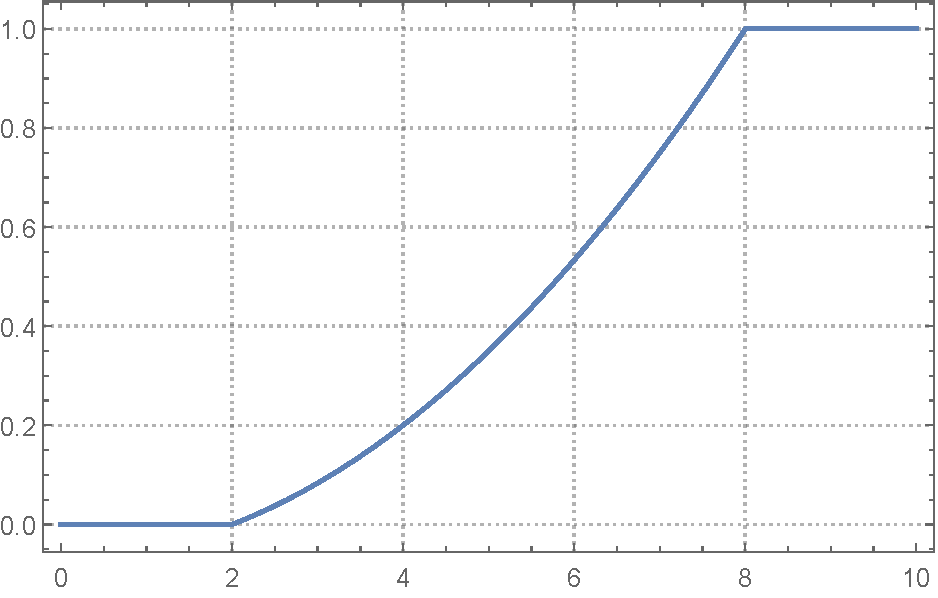
\includegraphics[width=7cm]{img_graph2} & 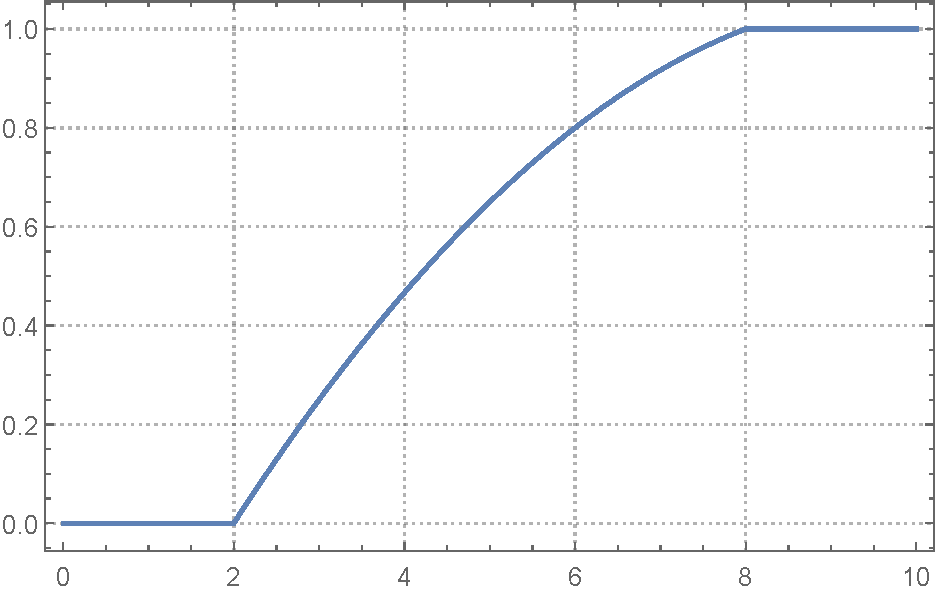
\includegraphics[width=7cm]{img_graph1} \\
		{\footnotesize Exemple de graphe pour $F(x)$ avec $y_0 < y_1$} & {\footnotesize Exemple de graphe pour $F(x)$ avec $y_0 > y_1$}
	\end{tabular}
\end{center}

La méthode des fonctions inverses consiste à utiliser la réciproque  $F^{-1}(y) : [0;1] \rightarrow [x_0;x_1]$ et une variable $y \sim \mathcal{U}(0, 1)$ pour déterminer une réalisation $x = F^{-1}(y)$ conforme à la densité de probabilité désirée pour $X$.

Dans le cas où $y_1 = y_0$, la solution est simple: la densité de probabilité définie par $f$ est une uniforme sur l'intervalle $[x_0;x_1]$ que l'on peut générer trivialement à partir d'une uniforme sur l'intervalle $[0,1]$:
\begin{equation*}
u \sim \mathcal{U}(a,b) = a + (b - a) \big( v \sim \mathcal{U}(0, 1) \big)
\end{equation*}

Dans le cas contraire, nous devons inverser $y = F(x)$ lorsque $x \in [x_0, x_1]$ et que $y_0 \ne y_1$:
\begingroup
\addtolength{\jot}{1em}
\begin{align*}
	y &= \frac{1}{y^2_1 - y^2_0} \cdot \left( \left( m_0 \cdot  \left( x - x_0 \right) + y_0 \right)^2 - y^2_0 \right) \\
	y \cdot (y_1^2 - y_0^2) + y^2_0 &=  \left( m_0 \cdot  \left( x - x_0 \right) + y_0 \right)^2\\
	\pm \sqrt{y \cdot (y_1^2 - y_0^2) + y^2_0} &=  m_0 \cdot  \left( x - x_0 \right) + y_0 \\
	\frac{\pm \sqrt{y \cdot (y_1^2 - y_0^2) + y^2_0} - y_0}{m_0} + x_0 &=  x
\end{align*}
\endgroup

Dans le cas contraire, nous devons déterminer le signe de la racine. La fonction $F(x)$ étant croissante, son inverse $F^{-1}(x)$ l'est également. Une étude des fonctions
\begin{align*}
	F^{-1}_a(y) &= \frac{+\sqrt{y \cdot (y_1^2 - y_0^2) + y^2_0} - y_0}{m_0} + x_0 \\
	F^{-1}_b(y) &= \frac{-\sqrt{y \cdot (y_1^2 - y_0^2) + y^2_0} - y_0}{m_0} + x_0
\end{align*}
révèle que la fonction $F^{-1}_a$ est croissante, alors que la fonction $F^{-1}_b$ est décroissante. Nous pouvons alors définir:
\begin{equation*}
	F^{-1}(y): [0;1] \rightarrow [x_0,x_1] = \left\lbrace \begin{array}{ll}
		x_0 + \frac{- y_0 + \sqrt{y \cdot (y_1^2 - y_0^2) + y^2_0}}{m_0}
		& \text{si $y_0 \ne y_1$} \\
		x_0 + y \cdot (x_1 - x_0)
		& \text{si $y_0 = y_1$}
	\end{array} \right.
\end{equation*}

L'algorithme de génération de réalisations est alors trivial:
\begin{enumerate}[1]
	\ttfamily
	\item Générer $y \sim \mathcal{U}(0, 1)$
	\item Retourner $F^{-1}(y)$
\end{enumerate}

\point{f}{\em Développer un algorithme permettant de générer des réalisations de la variable $X$ à l'aide d'une approche géométrique basée sur la méthode d'acceptation-rejet et en utilisant efficacement les symétries.}

La méthode d'acceptation-rejet consiste à \emph{enfermer} notre fonction de densité $f(x)$ sous une fonction de densité $g(x)$ plus simple tel que $\forall x \in [x_0,x_1], f(x) \leq c \cdot g(x) \mid c \in \mathbb{R}$ pour laquelle nous savons générer des réalisations aléatoires. Nous retournerons alors des réalisations $y \sim g$ si $\mathcal{U}(0,1) \leq \frac{f(y)}{cg(y)}$.

Dans notre cas, il n'est même pas nécessaire de respecter strictement le concept de fonction de densité et nous pouvons utiliser directement $\tilde{f}$ et une borne supérieure $y_m=y_0+y_1$, puis générer des réalisations $(a,b) \mid a \sim \mathcal{U}(x_0, x_1), b \sim \mathcal{U}(0, y_m)$ qui correspondent à des points uniformément distribués dans le rectangle sous la courbe de la fonction $g(x)=y_0+y_1$ sur l'intervalle $[x_0, x_1]$.

\begin{center}\small
	\renewcommand{\pshlabel}[1]{\scriptsize $#1$}
	\renewcommand{\psvlabel}[1]{\scriptsize $#1$}
	\psset{unit=1.5cm,linecolor=black,linewidth=0.5pt,fillstyle=none}
	\begin{pspicture}(-0.5,-1)(3.5,3)
	\psaxes[labels=none,ticks=none]{->}(0,0)(-0.25,-0.25)(3.5,2.5)
	\uput[-90](3.5,0){$x$}
	\uput[0](0,2.5){$\tilde{f}(x)$}
	\psline[linestyle=dashed](0,0.75)(1,0.75)
	\psline[linestyle=dashed](0,1.5)(2.5,1.5)
	\psset{labelsep=6pt}
	\uput[-90](1,0){$x_0$}
	\uput[-90](2.5,0){$x_1$}
	\psset{labelsep=3pt}
	\uput[180](0,0.75){$y_0$}
	\uput[180](0,1.5){$y_1$}
	
	
	\uput[180](0,2.25){$y_m$}
	\psline[linestyle=dashed](0,2.25)(1,2.25)
	
	\psset{linecolor=red,linewidth=1.5pt}
	\psline{-o}(-0.5,0)(1,0)
	\psline{*-*}(1,0.75)(2.5,1.5)
	\psline{o-}(2.5,0)(3.4,0)
	
	\psset{linecolor=blue,linewidth=0.5pt}
	\psline(1,0)(1,2.25)
	\psline(1,2.25)(2.5,2.25)
	\psline(2.5,2.25)(2.5,0)
	
	\end{pspicture}
\end{center}

Nous retournerons alors $a$ si $b \leq \tilde{f}(a)$ est vérifié. Dans le cas contraire, de nouvelles réalisations de $a$ et $b$ devront être générées jusqu'à vérifier l'inégalité.

Cependant, puisque le segment $\big\lbrace (x_0,y_0) , (x_1,y_1) \big\rbrace$ délimitant l'aire de la fonction $\tilde{f}$ divise le rectangle $\big\lbrace (x_0,0) , (x_1,0) , (x_1,y_0+y_1) , (x_0,y_0+y_1) \big\rbrace$ en deux parts égales, il est possible de \emph{rattraper le coup} lorsque le point $(a,b)$ est en dehors de l'aire de $\tilde{f}$ en effectuant une symétrie par rapport au centre du rectangle pour déplacer un point tombé dans la mauvaise part du rectangle.

\begin{center}
	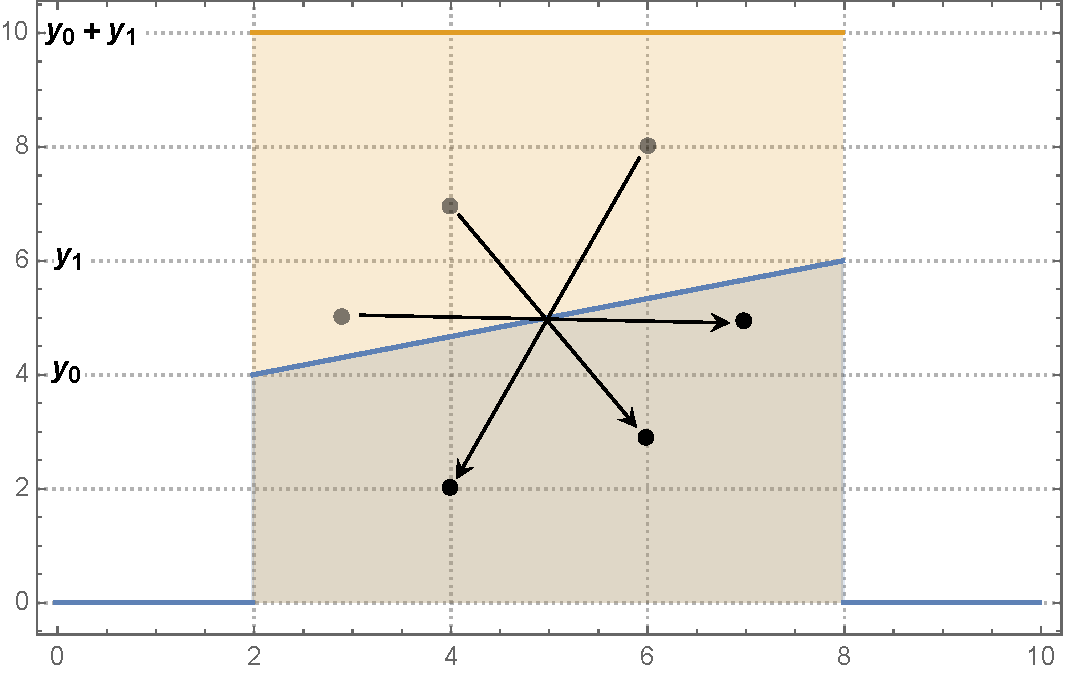
\includegraphics[width=8cm]{img_graph4}\\
	{\footnotesize Récupération de points dans la mauvaise part}
\end{center}

Nous avons donc l'algorithme suivant, sans possibilité de rejet:

\fbox{\parbox{16.2cm}{
\begin{enumerate}[\hspace{5mm}1 ]
	\ttfamily
	\item Générer $a \sim \mathcal{U}(x_0,x_1)$ et $b \sim \mathcal{U}(0,y_0+y_1)$
	\item Si $b \leq \tilde{f}(a)$ alors
	\item \tab // Dans l'aire de $\tilde{f}(x)$
	\item \tab Retourner $a$
	\item Sinon
	\item \tab // Hors de l'aire de $\tilde{f}(x)$, on prend la symétrie
	\item \tab Retourner $x_1 - (a - x_0)$
	\item Fin
\end{enumerate}}}

\pagebreak
\exo
	
{\em Déterminer la constante $A$ telle que $f=\frac{1}{A}\tilde{f}$ soit une densité}

Idem que pour le premier problème, nous cherchons ici $A = \int_{-\infty}^{\infty} \tilde{f}(x)\,dx$, soit l'aire sous la courbe de notre fonction $\tilde{f}$ afin de réduire cette aire à 1. À nouveau, chaque tranche de la fonction est un trapèze rectangle dont l'aire peut être calculée facilement.
\begin{align*}
	A &= \int_{a}^{b} \tilde{f}(x)\,dx \\
	  &= \sum_{k=0}^{n-1} \int_{x_k}^{x_{k+1}} \tilde{f}(x)\,dx \\
	  &= \sum_{k=0}^{n-1} \frac{(y_{k+1} + y_k)}{2}(x_{k+1}-x_k) \\
	  &= \frac{1}{2} \sum_{k=0}^{n-1} (y_{k+1} + y_k)(x_{k+1}-x_k)
\end{align*}

{\em Développer un algorithme pour générer des réalisations de la variable $X$ basé sur une application directe, "bête et méchante", de la méthode d'acceptation-rejet.}

La première étape consiste à déterminer le maximum $y_m$ de la fonction $\tilde{f}(x)$. Ce maximum correspond nécessairement à une valeur $y_k$ pour $k \in \lbrace 0,1,2,\dots,n \rbrace$.

Nous générons ensuite deux variables aléatoires $(x, y)$ indépendantes selon une loi uniforme, une fois sur l'intervalle $[a,b]$ et une fois sur l'intervalle $[0,y_m]$. Le couple $(x,y)$ de chaque tirage correspond à un point aléatoire dans le rectangle enfermant le graphe de la fonction $\tilde{f}$.

La dernière étape est de vérifier que $b \leq \tilde{f}(a)$, c'est à dire que le point $P(x, y)$ se situe sous la courbe de $\tilde{f}$. Si ce n'est pas le cas, nous effectuons un nouveau tirage des variables $x$ et $y$, jusqu'à ce que la condition soit vérifiée.

\fbox{\parbox{16.75cm}{
{\bf \vspace{2mm} Algorithme 2.b}
\begin{enumerate}[\hspace{2.5mm}1 ]
	\ttfamily
	\item Définir $y_m=\max(y_0, y_1, \dots, y_k)$
	\item Générer $x \sim \mathcal{U}(a,b)$ et $y \sim \mathcal{U}(0,y_m)$
	\item Si $y \leq \tilde{f}(x)$ alors
	\item \tab Retourner $x$
	\item Sinon
	\item \tab Sauter à la ligne 2
	\item Fin
\end{enumerate}}}

{\em Développer un algorithme pour générer des réalisations de la variable $X$ basé sur la méthode des mélanges et sur la méthode développée au point f) du problème précédent.}

Un des concepts de la méthode des mélanges est d'associer à chaque élément une probabilité $p_k$ proportionnelle à la part d'impact de l'élément sur l'ensemble du mélange et $\sum_{k=0}^{n-1} p_k = 1$.

Dans notre cas, nous associons à la $k$-ième tranche de $\tilde{f}$ une probabilité $p_k$ égale au rapport entre l'aire sous la courbe sur l'intervalle $[x_k,x_{k+1}]$ et l'aire totale sous la courbe de la fonction $\tilde{f}$.

Par la suite, nous générons un indice $j$ obéissant à la loi discrète
$P(j=k)=p_k \mid k=0,\dots,n-1$.

Une fois la tranche choisie, nous pouvons appliquer l'algorithme du point 1.f avec quelques substitutions pour correspondre au contexte de ce problème.

\algo{Algorithme 2.c}{
	\item Pour $k=0$ jusqu'à $n-1$:
	\item \tab Définir $\tilde{f}_k =
		\left\lbrace \begin{array}{ll}
			\tilde{f}(x) 	& \text{si $x_k \le x \le x_{k+1}$} \\
			0 				& \text{sinon}
		\end{array} \right.$ \\
	\item \tab Définir $p_k = \cfrac{\int_{x_k}^{x_{k+1}} \tilde{f}_k(x)\,dx}{A} = \cfrac{(x_{k+1}-x_k)(y_{k+1}+y_k)}{2A}$
	\item Définir $F_0 = p_0$
	\item Pour $k=1$ jusqu'à $n-1$:
	\item \tab Définir $F_k = F_{k-1}+p_k$
	\item Générer $u \sim \mathcal{U}(0, 1)$ et définir $j=0$, l'indice d'une section de $\tilde{f}$
	\item Répéter
	\item \tab Si $u \le F_j$, définir $t=j$ et quitter la boucle
	\item \tab Sinon, incrémenter $j$
	\item Appliquer l'algorithme 1.f sur la tranche $[x_j;x_{j+1}]$ de la fonction $\tilde{f}$, avec:
	\item \tab // Substitutions dans l'algorithme du point 1.f...
	\item \tab $x_0,\,x_1 = x_j,\,x_{j+1}$
	\item \tab $y_0,\,y_1 = y_j,\,y_{j+1}$
	\item \tab $\tilde{f}(x) = \tilde{f}_j(x)$
}

\begin{center}\small
	\renewcommand{\pshlabel}[1]{\scriptsize $#1$}
	\renewcommand{\psvlabel}[1]{\scriptsize $#1$}
	\psset{unit=1.5cm,linecolor=black,linewidth=0.5pt,fillstyle=none}
	\begin{pspicture}(-0.5,-0.5)(8,3.25)
	\psaxes[labels=none,ticks=none]{->}(0,0)(-0.25,-0.25)(8,3)
	\uput[-90](8,0){$x$}
	\uput[0](0,3){$\tilde{f}(x)$}
	\psline[linestyle=dashed](1,0)(1,0.75)(0,0.75)
	\psline[linestyle=dashed](2,0)(2,1.5)(0,1.5)
	\psline[linestyle=dashed](2.75,0)(2.75,2.5)(0,2.5)
	\psline[linestyle=dashed](3.5,0)(3.5,2)
	\psline[linestyle=dashed](6,0)(6,1.75)
	\psline[linestyle=dashed](7,0)(7,1)
	\psset{labelsep=6pt}
	\uput[-90](1,0){$x_0=a$}
	\uput[-90](2,0){$x_1$}
	\uput[-90](2.75,0){$x_2$}
	\uput[-90](3.5,0){$x_3$}
	\uput[-90](6,0){$x_{n-1}$}
	\psset{labelsep=4pt}
	\uput[-90](7,0){$x_n=b$}
	\psset{labelsep=3pt}
	\uput[180](0,0.75){$y_0$}
	\uput[180](0,1.5){$y_1$}
	\uput[180](0,2.5){$y_2$}
	\psset{linecolor=red,linewidth=1.5pt}
	\psline{-o}(-0.5,0)(1,0)
	\psline{*-*}(1,0.75)(2,1.5)
	\psline{*-*}(2,1.5)(2.75,2.5)
	\psline{*-*}(2.75,2.5)(3.5,2)
	\psline[linestyle=dashed]{*-}(3.5,2)(4,2)
	\psline[linestyle=dashed]{-*}(5.5,2.5)(6,1.75)
	\psline{*-*}(6,1.75)(7,1)
	\psline{o-}(7,0)(7.9,0)
	\end{pspicture}
\end{center}

foo

\begin{center}\small
	\renewcommand{\pshlabel}[1]{\scriptsize $#1$}
	\renewcommand{\psvlabel}[1]{\scriptsize $#1$}
	\psset{unit=1.5cm,linecolor=black,linewidth=0.5pt,fillstyle=none}
	\begin{pspicture}(-1,-1)(3.5,3)
	\psaxes[labels=none,ticks=none]{->}(0,0)(-0.25,-0.25)(3.5,2.5)
	\uput[-90](3.5,0){$x$}
	\uput[0](0,2.5){$\tilde{f}(x)$}
	\psline[linestyle=dashed](0,0.75)(1,0.75)
	\psline[linestyle=dashed](0,1.5)(2.5,1.5)
	\psset{labelsep=6pt}
	\uput[-90](1,0){$x_0$}
	\uput[-90](2.5,0){$x_1$}
	\psset{labelsep=3pt}
	\uput[180](0,0.75){$y_0$}
	\uput[180](0,1.5){$y_1$}
	
	
	\uput[180](0,2.25){$y_1+y_0$}
	\psline[linestyle=dashed](0,2.25)(1,2.25)
	
	\psset{linecolor=red,linewidth=1.5pt}
	\psline{-o}(-0.5,0)(1,0)
	\psline{*-*}(1,0.75)(2.5,1.5)
	\psline{o-}(2.5,0)(3.4,0)
	
	\psset{linecolor=blue,linewidth=0.5pt}
	\psline(1,0)(1,2.25)
	\psline(1,2.25)(2.5,2.25)
	\psline(2.5,2.25)(2.5,0)
	
	\end{pspicture}
\end{center}

foo


\end{document}